\documentclass{article}
\usepackage[margin=1in]{geometry}
\usepackage{listings}
\usepackage{problemset}

% Configure listings for Python syntax highlighting
\lstset{
    language=Python,
    basicstyle=\ttfamily\small,
    keywordstyle=\color{blue}\bfseries,
    showstringspaces=false,
    breaklines=true,
    numbers=left,
    numberstyle=\tiny\color{black},
    stepnumber=1,
    numbersep=5pt
}
\showsolntrue

% Custom commands
\newcommand{\R}{\mathbb{R}}
\newcommand{\X}{\mathcal{X}}
\newcommand{\Y}{\mathcal{Y}}
\newcommand{\E}{\mathbb{E}}
\newcommand{\V}{\text{Var}}
\newcommand{\C}{\text{Cov}}

\begin{document}

\pstitle{%
    DSC 140A%
}{
    Homework 2%
}[due Wednesday, October 22 at 11:59PM]

\begin{probset}
\begin{prob} [\textbf{Testing Linear Regression with Synthetic Datasets}]
    \textit{\textcolor{blue}{\textbf{Motivation:} In this problem, we'll work with linear regression model with two input variables x1 and x2. Our goal is to show you how the probabilistic assumptions for linear regression can be expressed in code, and you can use synthetic dataset to understand how models when various assumptions are violated.}}

    Create a dataset of $n = 100$ points for a 2D regression task using the following code snippet.

    \begin{lstlisting}
import numpy as np
def generate_dataset(n = 100, seed = 140):
    np.random.seed(seed)
    X1 = np.random.uniform(0,1,n)
    U = np.random.uniform(0,1,n)
    X2 = 0.5 * X1 + 10*U
    E = np.random.normal(0,1,n)
    Y = 2 * X1 + 0.3 * X2 + E
    return X1, X2, Y
    \end{lstlisting}

    \begin{subprobset}
        \begin{subprob}
            Say we were to fit a linear regression on this dataset. Inspect the code snippet to determine the expected values of the coefficients $\E(\hat{w}_0), \E(\hat{w}_1)$ and $\E(\hat{w}_2)$? Your answer should state these values and explain why are correct.

            \begin{soln}
                Since $Y = 2 * X1 + 0.3 * X2 + E$, we can expect $\E(\hat{w}_0) = \E(E) = 0$ since $E$ is normally distributed with mean 0. We can also expect $\E(\hat{w}_1) = 2$ and $\E(\hat{w}_2) = 0.3$ since $Y$ is calculated using those coefficients.
            \end{soln}
        \end{subprob}

        \begin{subprob}
            Generate a dataset with 100 points by calling \texttt{generate\_dataset(n = 100, seed = 140)}. Use your dataset to fit a linear regression model to predict $y$ from $x_1$ and $x_2$.

            \begin{enumerate}[label=\roman*.]
                \item Compare the values of $\hat{w}_0, \hat{w}_1, \hat{w}_2$ to their true values in Part (1). Explain the reason for
                any discrepancies you observe. Confirm your answer by generating a different dataset.
                \item Can you reject the null hypothesis $H_0 : w_1 = 0$ at a significance level of 5\%? How about
                $H_0 : w_2 = 0$?
            \end{enumerate}

            \begin{soln}
                On my first run, I got $\hat{w}_0 = 0.134$, $\hat{w}_1 = 2.41$, and $\hat{w}_2 = 0.259$. Setting the seed to 42, I got $\hat{w}_0 = -0.09$, $\hat{w}_1 = 1.62$, and $\hat{w}_2 = 0.37$. The discrepancies are due to the fact that there is a normally distributed error term being added to $Y$ upon generation. If there were no error term i.e. $Y = 2 * X1 + 0.3 * X2$, the coefficients would be exactly the same as the true values.

                To test the null hypotheses, let $H_a: w_i \neq 0$. We can use the t-test to test these hypotheses. The t-statistic is given by:
                \[ t_i = \frac{\hat{w}_i - 0}{\sqrt{\V(\hat{w}_i)}} \]
                where $\V(\hat{w}_i) = \frac{(X^T X)^{-1}_{ii}}{n - d - 1}\sum_{i=1}^n (y_i - \hat{y}_i)^2$. We can then find the p-values with:
                \[ p_i = 2 * (1 - \texttt{stats.t.cdf}(\texttt{np.abs}(t_i), df=n-d-1)) \]
                If the p-value is less than 0.05, we reject the null hypothesis. Since I got $p_1 = 0.000004$ and $p_2 = 0$, we can reject the null hypothesis for both $w_1$ and $w_2$.
            \end{soln}
        \end{subprob}

        \begin{subprob}
            Generate 1000 datasets for random seed values of \texttt{seed in range(1000)}, fit a linear model on each dataset, and collect the results.

            \begin{enumerate}[label=\roman*.]
                \item Use your results to plot the joint distribution of estimated coefficients ($\hat{w}_1, \hat{w}_2$) for each model.
                \item Use your results to report 95\% confidence intervals for each coefficient. Your answer should state the intervals, and a statement of what they mean in words.
                \item Use your results to evaluate the reliability of your conclusions from Part (2). Do your estimates appear reasonable? How about the results of your hypothesis tests?
            \end{enumerate}

            \begin{soln}
                \begin{center}
                    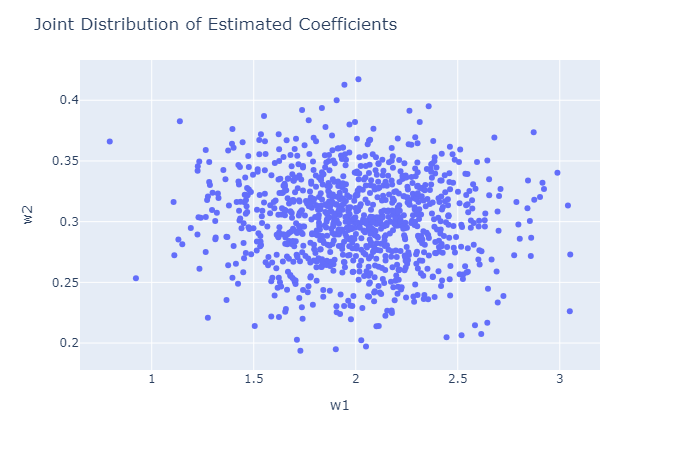
\includegraphics[width=0.9\textwidth]{Images/1.3.png}
                \end{center}

                The 95\% confidence intervals are $[-0.542151, 0.527369]$ for $w_0$, $[ 1.31597, 2.682614]$ for $w_1$ and $[ 0.23085, 0.371991]$ for $w_2$. These intervals indicate that we are 95\% confident that the true values of $w_1$ and $w_2$ are within these intervals.

                Considering that the intervals do not contain 0, we can again reject both null hypotheses $H_0 : w_1 = 0$ and $H_0 : w_2 = 0$ at a significance level of 5\%.
            \end{soln}
        \end{subprob}

        \newpage

        \begin{subprob}
            We'll now use following function to generate datasets that violate key assumptions for valid inference and test how they affect inference.

            \begin{lstlisting}
import numpy as np
def generate_dataset_for_failure(n = 100, seed = 140):
    np.random.seed(seed)

    ### START CODE ###
    X1 = np.random.uniform(0,1,n)
    U = np.random.uniform(0,1,n)
    X2 = 0.5 * X1 + 10*U
    E = np.random.normal(0,1,n)
    ### END CODE ###

    Y = 2 * X1 + 0.3 * X2 + E
    return X1, X2, Y
            \end{lstlisting}

            Each of the following functions will only require you to change 1-2 lines of code above. Make sure to edit the code only between the \texttt{\#\#\# START CODE \#\#\#} and \texttt{\#\#\# END CODE \#\#\#}, and share the entire function in your answer. You can then test the reliability by running the code snippet for $m = 100$ different random seeds by using a code snippet like below, and seeing if you fail to reject $H_0 : w_1 = 0$ and $H_0 : w_2 = 0$.

            \begin{lstlisting}
m = 100
for seed in range(m):
    X1, X2, Y = generate_dataset_for_failure(n=100, seed=seed)
    # Rest of your code
            \end{lstlisting}

            \begin{enumerate}[label=\roman*.]
                \item Set the value of the error term so that you consistently \textbf{fail to reject} $H_0 : w_1 = 0$ across
                multiple plausible datasets. Confirm your solution by reporting the false discovery rate
                when generating data using the original function and comparing it with the data generated
                by your modified version.
                \item Generate a dataset that violates the \textbf{full rank} assumption (i.e., that the columns of $X$ are
                linearly independent). Check to see how this affects the reliability of inference by testing
                $H_0 : w_1 = 0$ and $H_0 : w_2 = 0$ on multiple realizations of the dataset.
                \item Generate a dataset that violates the \textbf{homoskedasticity} assumption (i.e., that the error
                variance is fixed across observations). Confirm the reliability of your solution by implementing the change and running the code snippet for different random seeds.
            \end{enumerate}

            \begin{soln}
                If you set the error term to have a standard deviation of 10 rather than 1, you will consistently fail to reject $H_0 : w_1 = 0$ across multiple plausible datasets. I tested the first function 100 times with a random seed and got a false discovery rate of 0\% while the second function had a false discovery rate of 100\%.

                You can violate the full rank assumption by setting $X2 = 5 - 5 * X1$. Although this has a false discovery rate of 0\% for $w_1$, it has a false discovery rate of 92\% for $w_2$.

                You can violate the homoskedasticity assumption by setting $E = E * \sqrt{X1}$. After testing the null 100 times with a random seed, I got a false discovery rate of 0\% so it seems like the inference is not affected. However, if you set $E = E / X1$, you will consistently reject the null hypothesis $H_0 : w_1 = 0$ with a false discovery rate of 100\%.
            \end{soln}
        \end{subprob}
    \end{subprobset}
\end{prob}

\newpage

\begin{prob} [\textbf{Pitfalls of Hidden Assumptions and Transformations}]
    \textit{\textcolor{blue}{\textbf{Motivation:} In this problem, we study the underlying assumptions for inference with linear regression. We'll work on a simple problem where there may not be a clear-cut answer. Our goal is to show how inference can fail when these assumptions are violated and how we can fix these issues by applying transformations.}}

    In this problem, we'll study the outputs of two models that were designed to study how global rice prices changed from 2003 to 2009. Here, each data point has the form $(x_i, y_i)$ where $x_i$ and $y_i$ encode the price of rice in city $i$ in 2003 and 2009, respectively. In Fig. 1, we show the raw data and best-fit lines for a standard model and a model with a \textbf{log-log} transformation.

    \begin{center}
        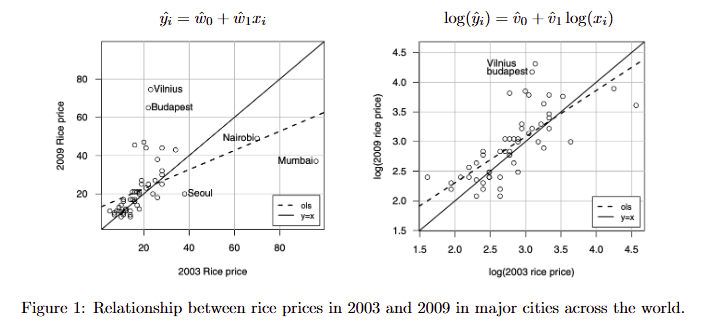
\includegraphics[width=0.9\textwidth]{Images/P2.png}
    \end{center}

    \begin{subprobset}
        \begin{subprob}
            This example shows that we can apply linear regression to transformations of the inputs and outputs. For each model above:

            \begin{enumerate}[label=\roman*.]
                \item State the underlying generative model $y_i | x_i$;
                \item Describe an expression for the maximum likelihood parameters;
                \item Describe how to interpret the intercept parameter, slope parameter, and error term.
            \end{enumerate}

            \begin{soln}
                For the first model, the generative model is $y_i | x_i \sim \text{Normal}(w_0 + w_1 x_i, \sigma^2)$. The maximum likelihood parameters are:
                \begin{align*}
                    \hat{w}_1 &= \frac{\sum_{i=1}^n (x_i - \bar{x})(y_i - \bar{y})}{\sum_{i=1}^n (x_i - \bar{x})^2} \\
                    \hat{w}_0 &= \bar{y} - \hat{w}_1 \bar{x}
                \end{align*}
                Where $\bar{x} = \frac{1}{n} \sum_{i=1}^n x_i$ and $\bar{y} = \frac{1}{n} \sum_{i=1}^n y_i$. The interpretation of the intercept parameter is the expected rice price in 2009 when the price of rice in 2003 is hypothetically 0. The interpretation of the slope parameter is the expected change in the price of rice in 2009 for each \$1 increase in the price of rice in 2003. The interpretation of the error term is the random variation around the linear relationship.
                
                For the second model, the generative model is $\log(y_i) | \log(x_i) \sim \text{Normal}(v_0 + v_1 \log(x_i), \sigma^2)$ which implies $y_i | x_i \sim \text{LogNormal}(v_0 + v_1 \log(x_i), \sigma^2)$. The maximum likelihood parameters are:
                \begin{align*}
                    \hat{v}_1 &= \frac{\sum_{i=1}^n (\log(x_i) - \tilde{x})(\log(y_i) - \tilde{y})}{\sum_{i=1}^n (\log(x_i) - \tilde{x})^2} \\
                    \hat{v}_0 &= \tilde{y} - \hat{v}_1 \tilde{x}
                \end{align*}
                Where $\tilde{x} = \frac{1}{n} \sum_{i=1}^n \log(x_i)$ and $\tilde{y} = \frac{1}{n} \sum_{i=1}^n \log(y_i)$. The interpretation of the intercept parameter is the expected log rice price in 2009 when the price of rice in 2003 is hypothetically 1. The interpretation of the slope parameter is the expected change in log rice price in 2009 for each unit increase in log rice price in 2003. The interpretation of the error term is the random variation in the log scale around the linear relationship.
            \end{soln}
        \end{subprob}

        \begin{subprob}
            Estimate the values of $\hat{w}_0$ and $\hat{w}_1$ from the best-fit line on the left plot in Fig. 1. Use these values to describe how rice prices have changed from 2003 to 2009?

            \begin{soln}
                Looking at the left plot, we can estimate $\hat{w}_0 = 15$ and $\hat{w}_1 = 0.5$ (from $x = 20$ and $x = 60$). This means that for every dollar increase in the price of rice in 2003, the price of rice in 2009 is expected to be half that amount plus 15. The intercept parameter represents the price of rice in 2009 when the price of rice in 2003 is hypothetically 0. This means that rice prices have generally increased if the price of rice was cheap in 2003 (less than \$20) but decreased if the price of rice was expensive in 2003 (more than \$20).
            \end{soln}
        \end{subprob}
        
        \begin{subprob}
            Estimate the values of $\hat{v}_0$ and $\hat{v}_1$ based on the best-fit line on the right Fig. 1. Use these values to describe how rice prices have changed from 2003 to 2009?

            \begin{soln}
                Looking at the right plot, we can estimate $\hat{v}_1 = 0.8$ (from $x = 1.5$ and $x = 4$) and $\hat{v}_0 = 0.7$ (using the slope and $x = 3.5$). This means that for every order of magnitude of the price of rice in 2003, the order of magnitude of rice in 2009 is expected to be 0.8 that amount plus 0.7 magnitudes more. The intercept parameter represents the order of magnitude of rice in 2009 when the price of rice in 2003 is hypothetically 0. This means that rice prices have generally increased if the price of rice was cheap in 2003 (less than \$30) but decreased if the price of rice was expensive in 2003 (more than \$30).
            \end{soln}
        \end{subprob}

        \begin{subprob}
            Inspect the data and fitted models in Fig. 1 to evaluate if each model satisfies the assumptions for valid inference we covered in class, i.e., the five Gauss-Markov Assumptions. For each model and each assumption, state “Holds”, “Violated”, or “Can't Tell” and briefly explain your claim. Given the assumptions, which model is preferable for inference?

            \begin{soln}
                \begin{itemize}
                    \item No Multicollinearity (Holds, Holds): Both models seem to satisfy this assumption since the data doesn't form any perfect lines.
                    \item Independence (Can't Tell, Can't Tell): Both models might satisfy this assumption since know how the price changed for one city doesn't affect how the price changed for another city. However, this may not be the case since cities in the same region may have similar price changes. So I'll leave this as can't tell.
                    \item Linearity (Holds, Holds): Both models also follow this assumption since the data looks linear.
                    \item Zero Conditional Mean (Violated, Holds): The right model seems to satisfy this assumption while the left model doesn't since there are more data points below the fitted line than above.
                    \item Homoskedasticity (Violated, Holds): The right model seems to satisfy this assumption while the left model does not since the data points are more spread out for higher values of $x$.
                \end{itemize}
                Since the right model satisfies all the assumptions, it is preferable for inference.
            \end{soln}
        \end{subprob}
    \end{subprobset}
\end{prob}

\newpage

\begin{prob} [\textbf{Inference with Omitted and Irrelevant Variables}]
    \textit{\textcolor{blue}{\textbf{Motivation:} Many real-world datasets will contain a random mix of variables. In practice, only some of the variables may be related to the outcome that we'd like to predict. Other variables may be unrelated. In this problem, we'll study how the coefficient estimates of linear regression model will change in this regime.}}

    Consider fitting a linear regression model using data sampled from the model:
    \begin{align}
        y = w_0 + w_1 x_1 + w_2 x_2 + \epsilon
    \end{align}

    \begin{subprobset}
        \begin{subprob}
            Say we fit a model on a dataset without measurements for $x_2$. In this case, each data point would have the form $(x_{i,1}, y_i)$. If the outcomes were generated from the model in (1), however, we would violate an assumption for valid inference and obtain a biased estimate of $\hat{w}_1$.

            \begin{enumerate}[label=\roman*.]
                \item State the assumption and explain why it is violated.
                \item Derive a closed-form expression for the bias in the estimate $\hat{w}_1$ in terms of the quantities: $\C(x_1, x_2)$, $\V(x_1)$, and $w_2$.
            \end{enumerate}

            \begin{soln}
                The Zero Conditional Mean assumption is violated when we omit $x_2$. If we fit the model $y = \beta_0 + \beta_1 x_1 + u$, then the total error is $u = w_2 x_2 + \epsilon$. When $\C(x_1, x_2) \neq 0$, we have $\E[u\mid x_1] = w_2\,\E[x_2\mid x_1] \neq 0$, so $u$ OLS is biased.

                The OLS slope from the regression of $y$ on $x_1$ only is
                \[
                    \hat{\beta}_1 = \frac{\C(x_1, y)}{\V(x_1)}
                    = \frac{\C\big(x_1,\; w_0 + w_1 x_1 + w_2 x_2 + \epsilon\big)}{\V(x_1)}
                    = w_1 + w_2\,\frac{\C(x_1, x_2)}{\V(x_1)} + \frac{\C(x_1,\epsilon)}{\V(x_1)}.
                \]
                Using $\C(x_1,\epsilon)=0$, the expected value is
                \[
                    \E[\hat{\beta}_1] = w_1 + w_2\,\frac{\C(x_1, x_2)}{\V(x_1)}.
                \]
                Therefore, the bias is
                \[
                    \text{Bias}(\hat w_1) = \E[\hat{\beta}_1] - w_1 = w_2\,\frac{\C(x_1, x_2)}{\V(x_1)}.
                \]
                This is nonzero whenever $w_2 \neq 0$ and $\C(x_1, x_2) \neq 0$.
            \end{soln}
        \end{subprob}

        \newpage

        \begin{subprob}
            Say that we fit a model using a dataset that includes $x_1$ and $x_2$ and a new variable $x_3$. Each data point now has the form $(x_{i,1}, x_{i,2}, x_{i,3}, y_i)$. However, the outcomes are still generated from the model in (1), which only depends on $x_1$ and $x_2$.

            \begin{enumerate}[label=\roman*.]
                \item Write an expression for the model we fit using this dataset.
                \item What is the expected value for the coefficient for $x_3$?
                \item Say that you fit a model on this dataset. Would you expect your estimate $\hat{w}_3$ to match its expected value $\E(\hat{w}_3)$? Provide a brief explanation for your answer.
                \item Say that we fit two models: one with $x_3$ and another without $x_3$. Will the models return different estimates for $x_1$ and $x_2$? For each model, state if the coefficient estimate for $x_1$ and $x_2$ be biased?
            \end{enumerate}

            \begin{soln}
                We fit $y = w_0 + w_1 x_1 + w_2 x_2 + w_3 x_3 + u$.
                Here the true data-generating process has $w_3 = 0$. Under the usual assumptions (no perfect multicollinearity, zero conditional mean, finite variance), OLS is unbiased, so $\E(\hat w_3) = w_3 = 0$. In a single sample we do not expect $\hat w_3$ to equal 0 exactly since sampling variation leads to $\hat w_3 \neq 0$.
                
                Comparing the models with and without $x_3$, both give unbiased estimates for $w_1$ and $w_2$ since the true model only depends on $x_1, x_2$. Including the irrelevant $x_3$ would increase the variances of $\hat w_1, \hat w_2$ if $x_3$ is correlated with $x_1$ or $x_2$. So estimates may differ sample-by-sample but neither model introduces bias in $\hat w_1$ or $\hat w_2$.
            \end{soln}
        \end{subprob}

        \begin{subprob}
            Your friend Rod wants to fit a model after dropping variables that are clearly irrelevant variables. Rod argues that this technique will help them understand the factors that drive $y$ without affecting inference.

            \begin{enumerate}[label=\roman*.]
                \item Should Rod be worried about missing variables given our result in Part 3.1?
                \item Should Rod be worried about irrelevant variables given the result in Part 3.2?
                \item Describe a simple test that Rod could perform to rule out the potential problems from missing variables?
            \end{enumerate}

            \begin{soln}
                Dropping relevant variables can violate the zero conditional mean assumption. If a dropped variable is correlated with included regressors, OLS estimates are biased.

                Adding irrelevant variables does not introduce bias, but it can inflate standard errors, especially if the added variables are correlated with included regressors. So estimates stay unbiased but less precise.

                He can use cross-validated Lasso as a screening step: run Lasso on a rich feature set, record variables selected consistently, then refit OLS on those and compare to the small model. Large coefficient shifts suggest that the variable should be dropped.
            \end{soln}
        \end{subprob}
    \end{subprobset}
\end{prob}

\newpage

\begin{prob} [\textbf{Linear Regression with Dummy Variables and Interaction Effects}]
    \textit{\textcolor{blue}{\textbf{Motivation:} We end with a hands-on modeling task where we'll fit validate linear regression models for
    a real-world dataset. We'll work with a dataset with a few meaningful features so that you can explore the
    relationships between variables and plot them.}}

    We will explore the association between cholesterol, age, and diabetes in a small dataset from the National Health and Nutrition Examination Survey (\href{https://www.dropbox.com/scl/fi/nv7j1y6yvdafke4tgahwk/chol_data.csv?rlkey=r0q2w3mlb7pcljavatbv71s1z&st=30oeue65&dl=0}{link}). This dataset contains $n = 500$ data points where each point $(x_{i,1}, x_{i,2}, y_i)$ records the following variables:

    \begin{itemize}
        \item \texttt{TotChol ($y_i$)}: Total Cholesterol Level in mmol/L for Participant $i$
        \item \texttt{Age ($x_{i,1}$)}: Age for Participant $i$ in years
        \item \texttt{Diabetes ($x_{i,2}$)}: Diabetes status, set as 1 if Participant $i$ has diabetes, 0 otherwise
    \end{itemize}

    Load the dataset and fit a linear regression model to predict TotChol using Age and Diabetes using the following code snippet.

    \begin{lstlisting}
import pandas as pd
import statsmodels.api as sm
df = pd.read_csv("chol_data.csv")
X = df[["Age", "Diabetes"]]
X = sm.add_constant(X)
y = df["TotChol"]
model = sm.OLS(y, X).fit()
print(model.summary())
    \end{lstlisting}

    \begin{subprobset}
        \begin{subprob}
            Explain the meaning of the following values in the summary table: $R^2$, Std Err, and $P > |t|$.

            \begin{soln}
                The $R^2$ value is 0.017 which means that 1.7\% of the variation in TotChol is explained by Age and Diabetes. The Std Err is the standard deviation of the coefficient estimates, i.e. how much they tend to deviate from the true value. The $P > |t|$ value is the p-value for the t-test for the null hypothesis that the coefficient is equal to 0. In this case, they are all less than 0.05 so we can reject the null hypothesis that the coefficients are equal to 0.
            \end{soln}
        \end{subprob}

        \begin{subprob}
            Write expressions of the linear model for individuals with and without diabetes.

            \begin{soln}
                The linear model for individuals with diabetes is $y = 4.4823 - 0.0075x_2$ where $x_2$ is Age. The linear model for individuals without diabetes is $y = 4.8 - 0.0075 x_2$.
            \end{soln}
        \end{subprob}

        \newpage

        \begin{subprob}
            Create a scatterplot of \texttt{Age} (x-axis) vs \texttt{TotChol} (y-axis). Plot the fitted regression lines for individuals with and without diabetes. Describe the relationship between the two lines.

            \begin{soln}
                \begin{center}
                    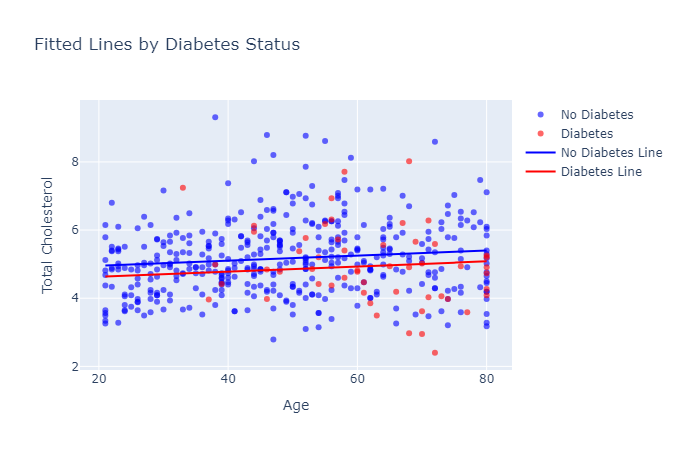
\includegraphics[width=0.9\textwidth]{Images/4.3.png}
                \end{center}
                The lines are parallel and increasing with age. This indicates that as age increases, Total Cholesterol tends to increase for both individuals with and without diabetes. However, since the blue line is above the red line, this means that individuals without diabetes generally have a higher Total Cholesterol than individuals with diabetes at any given age.
            \end{soln}
        \end{subprob}

        \newpage

        \begin{subprob}
            Add confidence and prediction intervals to your plot. Report the confidence and prediction intervals for $Age = 45$ and provide a one-sentence interpretation of what each interval means.

            \begin{soln}
                \begin{center}
                    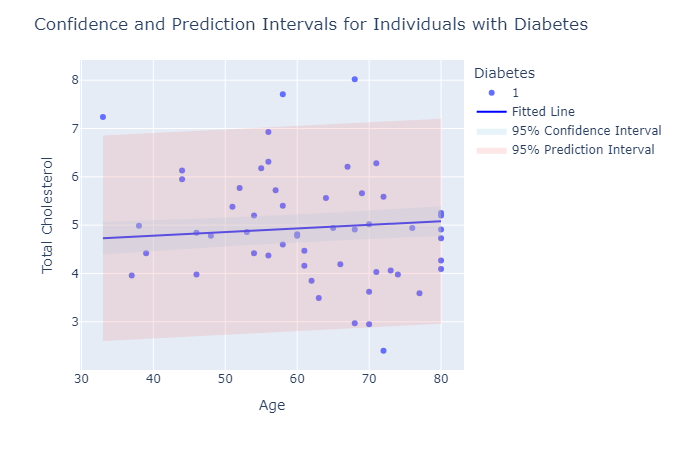
\includegraphics[width=0.9\textwidth]{Images/4.4a.png}
                    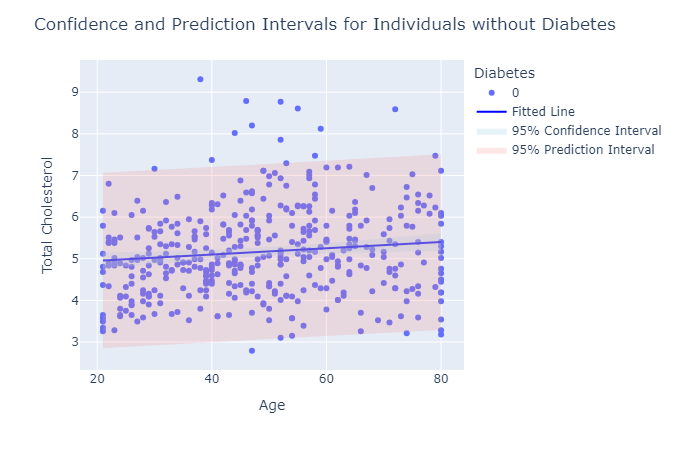
\includegraphics[width=0.9\textwidth]{Images/4.4b.png}
                \end{center}
                For individuals with diabetes, the confidence interval is [4.514, 5.124] and the prediction interval is [2.698, 6.941]. For individuals without diabetes, the confidence interval is [5.032, 5.241] and the prediction interval is [3.035, 7.239]. The confidence interval contains the expected value of Total Cholesterol with probability 95\% for the given age while the prediction interval contains the individual's Total Cholesterol with probability 95\% for the given age.
            \end{soln}
        \end{subprob}

        \begin{subprob}
            Plot the residuals against \texttt{Age}. Can you support the probabilistic assumptions in your case?

            \begin{soln}
                \begin{center}
                    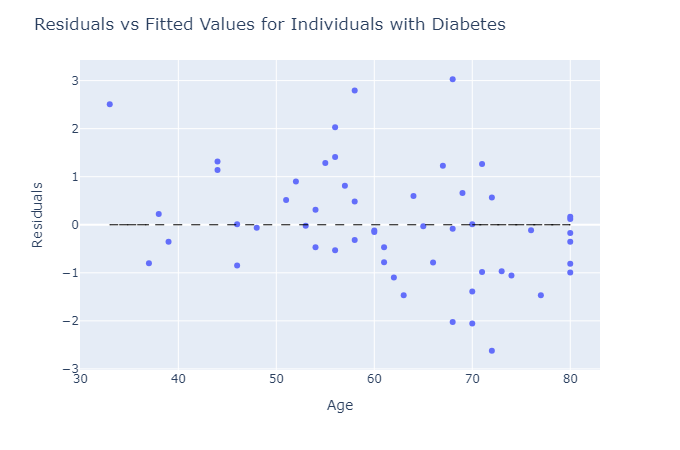
\includegraphics[width=0.85\textwidth]{Images/4.5a.png}
                    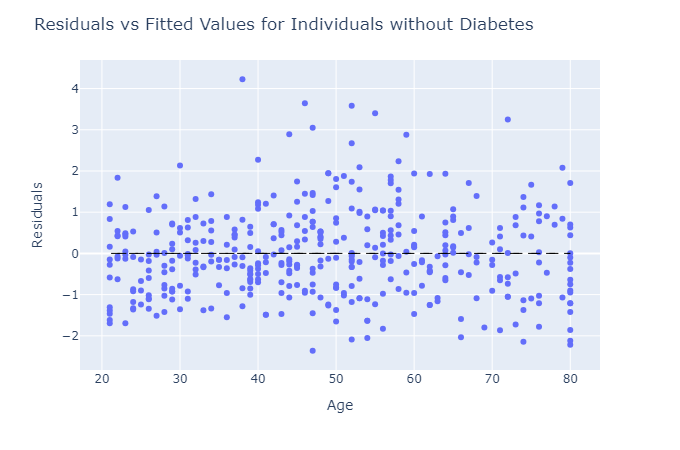
\includegraphics[width=0.85\textwidth]{Images/4.5b.png}
                \end{center}
                The data looks roughly linear for both plots, and independence should hold since knowing the Age and TotChol for one individual doesn't affect another, and the data isn't multicollinear. However, the zero conditional mean assumption and homoskedasticity are violated on the first plot since the residuals are not centered around 0 and the variance is not constant, especially for higher ages. So it's not reasonable to assume that the probabilistic assumptions are satisfied.
                On the second plot however, the residuals are centered around 0 and the variance is roughly constant, so it's reasonable to assume that the probabilistic assumptions are satisfied.
            \end{soln}
        \end{subprob}

        \newpage

        Linear regression models can allow the \textit{relationship} between the outcome and a specific variable to change depending on a categorical variable. Consider the model:

        \[ \E (\texttt{TotChol}) = w0 + w1 \cdot \texttt{Age} + w2 \cdot \texttt{Diabetes} + w3 \cdot (\texttt{Age} \times \texttt{Diabetes}) + \epsilon \]

        Here, \texttt{Age} $\times$ \texttt{Diabetes} is an interaction term where the coefficient $w_3$ allows the model to capture different effects of age on cholesterol based on their diabetes status.

        \begin{subprob}
            Repeat your analysis from Parts (a) to (e) for this new model. \textit{\textcolor{blue}{Note: you can reuse your code to
            fit the model and generate plots by adding a new feature to your dataset (\texttt{Age} $\times$ \texttt{Diabetes}).}}

            \begin{soln}
                For this model, the $R^2$ value is 0.032 which means that 3.2\% of the variation in TotChol is explained by Age, Diabetes, and the interaction term. The Std Err is the standard deviation of the coefficient estimates, i.e. how much they tend to deviate from the true value. The $P > |t|$ value is the p-value for the t-test for the null hypothesis that the coefficient is equal to 0. In this case, they are all less than 0.05 so we can reject the null hypothesis that the coefficients are equal to 0. 
                
                The linear model with diabetes is given to us as $y = 6.4144 + 0.0239\texttt{Age}$ and the linear model without diabetes is given to us as $y = 4.6957 + 0.0096\texttt{Age}$.

                \begin{center}
                    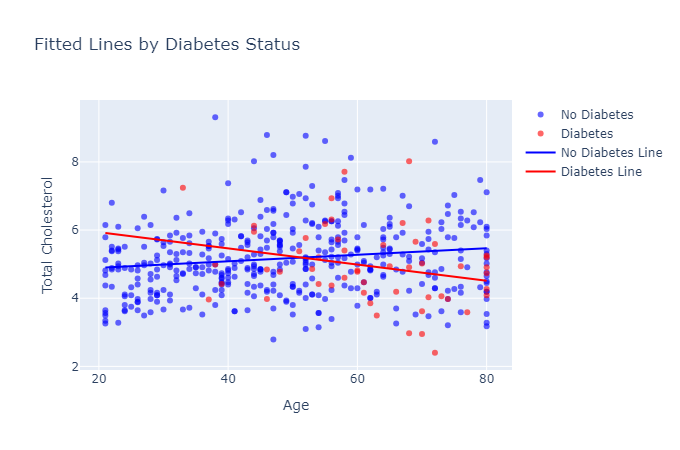
\includegraphics[width=0.8\textwidth]{Images/4.6a.png}
                \end{center}
                For individuals with diabetes, Total Cholesterol tends to be lower with increasing age. For individuals without diabetes, Total Cholesterol tends to be higher with increasing age.

                \begin{center}
                    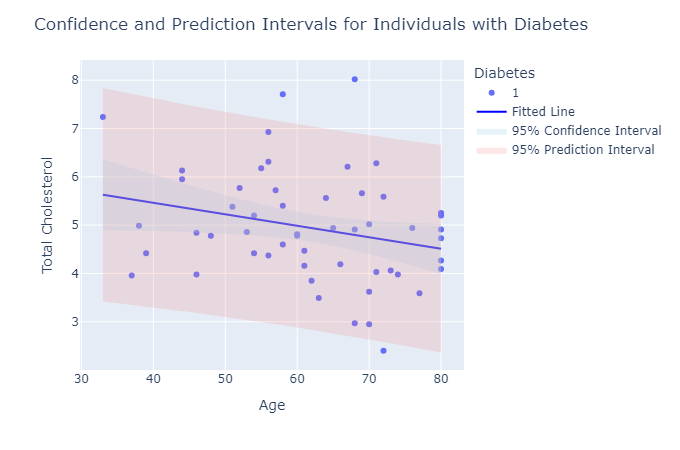
\includegraphics[width=0.8\textwidth]{Images/4.6b.png}
                    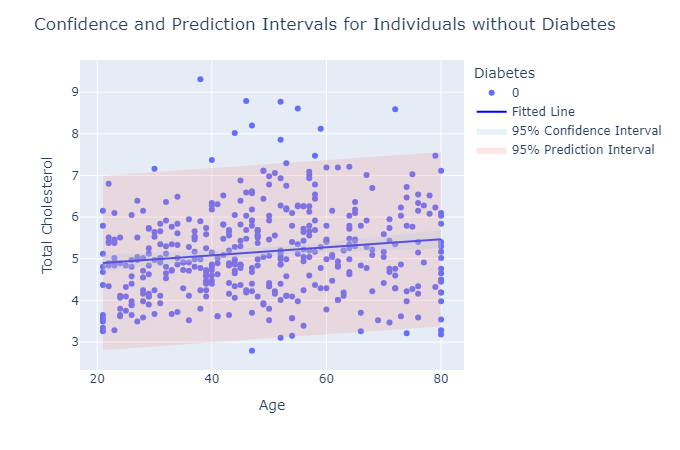
\includegraphics[width=0.8\textwidth]{Images/4.6c.png}
                \end{center}
                For individuals with diabetes at age 45, the confidence interval is [4.859, 5.827] and the prediction interval is [3.202, 7.483]. For individuals without diabetes at age 45, the confidence interval is [5.025, 5.234] and the prediction interval is [3.042, 7.217]. Interestingly, the trend line seems to fit the Diabetes better than the last model.

                \begin{center}
                    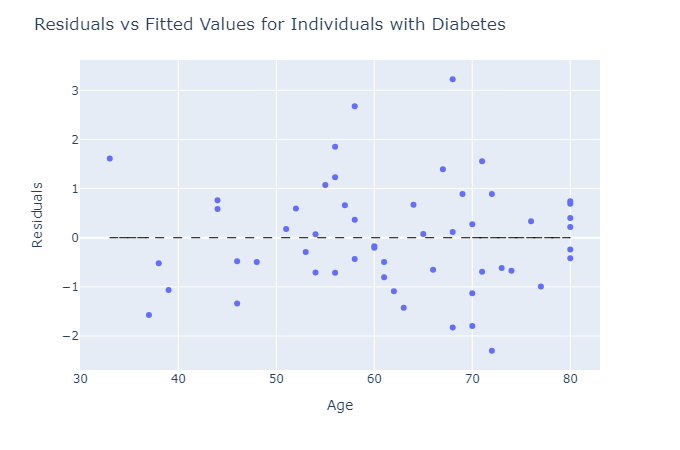
\includegraphics[width=0.8\textwidth]{Images/4.6d.png}
                    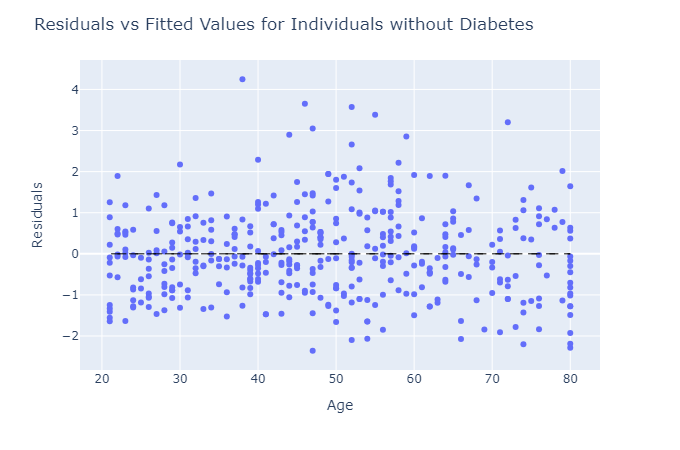
\includegraphics[width=0.8\textwidth]{Images/4.6e.png}
                \end{center}
                The data looks roughly linear for both plots, and independence should hold since knowing the Age and TotChol for one individual doesn't affect another, and the data isn't multicollinear. Although homoskedasticity is questionable on the first plot, it's not too bad, and the zero conditional mean assumption hold so the probabilistic assumptions are reasonably satisfied for both plots this time.
            \end{soln}
        \end{subprob}
    \end{subprobset}
\end{prob}

\begin{prob}[\textbf{Complete the Google form at the following \href{https://forms.gle/N46J26RMSZMeBx7q8}{link}.}]
    Responding to this form is \textbf{MANDATORY} as it is worth a few points. Please note that it's not the content that is graded but whether you filled the form or not.
\end{prob}
\end{probset}
\end{document}